\documentclass[11pt]{article}
\usepackage{preamble}
\titleformat*{\section}{\Large\bfseries}
\usepackage{mathtools}
\usepackage{listings, courier}
\lstset{basicstyle=\small\ttfamily,breaklines=true}
\lstset{
      numbers=left,
      stepnumber=1,    
      firstnumber=1,
      numberfirstline=true,
      xleftmargin=6em,
      framexleftmargin=3.5em,
      framextopmargin=6pt,
      framexbottommargin=6pt, 
      frame=tb, framerule=0pt,  
      numberstyle=\small\color{gray},
      numbersep=20pt,
      backgroundcolor=\color{gray!10},
}
\DeclarePairedDelimiter\ceil{\lceil}{\rceil}
\DeclarePairedDelimiter\floor{\lfloor}{\rfloor}
\def\columnseprulecolor{\color{blue}}

\title{CISC 3220 Homework Chapter 12}
\author{Rachel Friedman}
\date{May 3, 2020}

\begin{document}
\maketitle

\section*{Exercises 12.1}\nointerlineskip
\noindent \rule{\linewidth}{0.01pt}\\

\subsubsection*{Question 12.1-1}\nointerlineskip
For the set of $\{ 1, 4, 5, 10, 16, 17, 21 \}$  of keys, draw binary search trees of heights 2, 3, 4, 5, and 6.\\

\begin{center}
\begin{multicols}{2}

\textbf{Height = 2}\\[12pt]
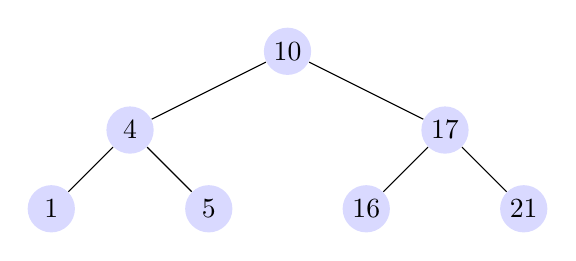
\begin{tikzpicture}
  [level distance = 10mm, node distance=0.1,
   every node/.style={fill=blue!15!white,circle, inner sep=1pt, minimum size=6mm},
   level 1/.style={sibling distance = 40mm},
   level 2/.style={sibling distance = 20mm},
   level 3/.style={sibling distance = 10mm}]
  \node {10}
     child {node{4}
       child {node {1}}
       child {node {5}}
     }
     child {node{17}
       child {node {16}}
       child {node {21}}
     };
\end{tikzpicture}

\columnbreak
\textbf{Height = 3}\\[12pt]
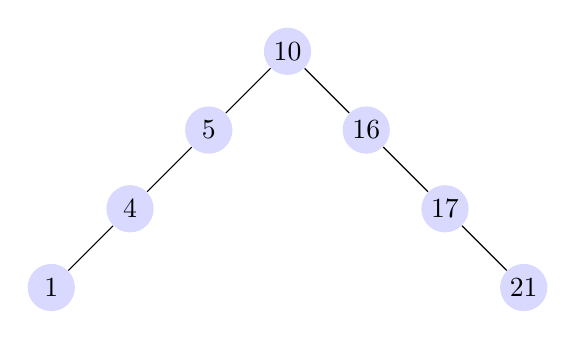
\begin{tikzpicture}
  [level distance = 10mm, node distance=0.1,
   every node/.style={fill=blue!15!white,circle, inner sep=1pt, minimum size=6mm},
   level 1/.style={sibling distance = 20mm},
   level 2/.style={sibling distance = 20mm},
   level 3/.style={sibling distance = 20mm}]
  \node {10}
     child {node{5}
        child {node {4}
            child {node {1}}
            child [missing]}
       child [missing]
     }
     child {node{16}
        child [missing]
        child {node {17}
            child [missing] 
            child {node {21}}}
     };
\end{tikzpicture}
\end{multicols}


\vspace{30pt}
\begin{multicols}{2}
\textbf{Height = 4}\\[12pt]
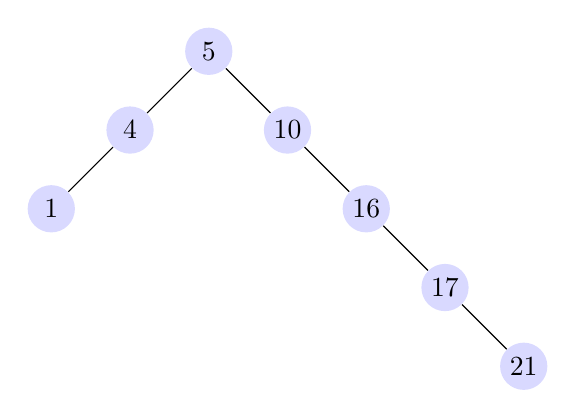
\begin{tikzpicture}
  [level distance = 10mm, node distance=0.1,
   every node/.style={fill=blue!15!white,circle, inner sep=1pt, minimum size=6mm},
   level 1/.style={sibling distance = 20mm},
   level 2/.style={sibling distance = 20mm},
   level 3/.style={sibling distance = 20mm}]
  \node {5}
     child {node{4}
        child {node {1}}
       child [missing]
     }
     child {node{10}
        child [missing]
        child {node {16}
            child [missing] 
            child {node {17}
                child [missing]
                child {node{21}}}
            }
     };
\end{tikzpicture}
\vspace{30pt}

\textbf{Height = 5}\\[12pt]
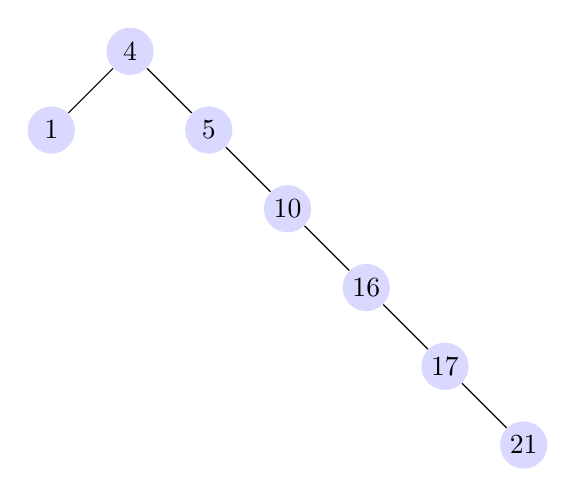
\begin{tikzpicture}
  [level distance = 10mm, node distance=0.1,
   every node/.style={fill=blue!15!white,circle, inner sep=1pt, minimum size=6mm},
   level 1/.style={sibling distance = 20mm},
   level 2/.style={sibling distance = 20mm},
   level 3/.style={sibling distance = 20mm}]
  \node {4}
     child {node{1}
       child [missing]
     }
     child {node{5}
        child [missing]
        child {node {10}
            child [missing] 
            child {node {16}
                child [missing]
                child {node{17}
                    child [missing]
                    child {node{21}}}
                }
            }
     };
\end{tikzpicture}
\end{multicols}
\vspace{30pt}
\newpage
\textbf{Height = 6}\\[12pt]
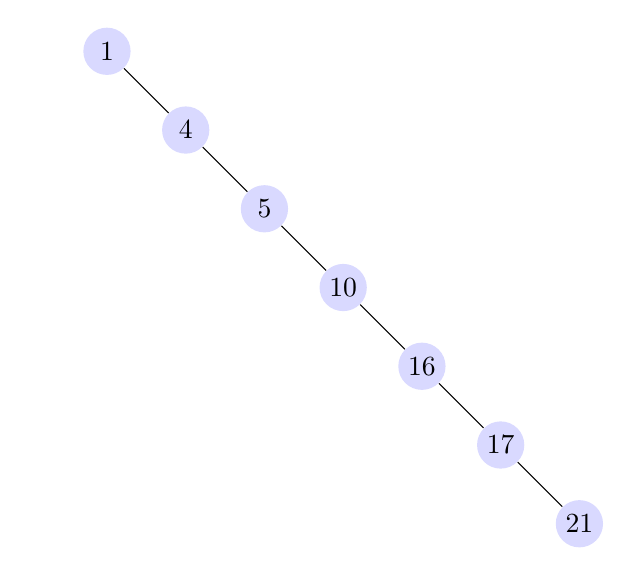
\begin{tikzpicture}
  [level distance = 10mm, node distance=0.1,
   every node/.style={fill=blue!15!white,circle, inner sep=1pt, minimum size=6mm},
   level 1/.style={sibling distance = 20mm},
   level 2/.style={sibling distance = 20mm},
   level 3/.style={sibling distance = 20mm}]
  \node {1}
     child [color=white]{[missing]
     }
     child {node{4}
        child [missing]
        child {node {5}
            child [missing] 
            child {node {10}
                child [missing]
                child {node{16}
                    child [missing]
                    child {node{17}
                        child [missing]
                        child {node{21}}}
                    }
                }
            }
     };
\end{tikzpicture}
\vspace{10pt}

\end{center}

\subsubsection*{Question 12.1-2}\nointerlineskip
What is the difference between the binary-search-tree property and the min-heap property? Can the min-heap property be used to print out the keys of an $n$-node tree in sorted order in $\mathcal{O}(n)$ time? \\

In a binary search tree, the left child is less than or equal to its parent and the right child is greater than or equal to its parent. In a min-heap tree, both the left and the right child are less than or equal to the parent, and the left child may be greater than the right child. For this reason, the min-heap tree cannot be printed in sorted order, because we have no way of knowing which subtree contains the next smallest element.\\

\subsubsection*{Question 12.1-4}\nointerlineskip
Give recursive algorithms that perform preorder and postorder tree walks in $\Theta(n)$ time on a tree of $n$ nodes.\\


\begin{minipage}{5in}
\begin{lstlisting}[language=Python]
def preorder_treewalk(node):
    if node != None:
        print(node.key)
        preorder_treewalk(node.left)
        preorder_treewalk(node.right)
        
def postorder_treewalk(node):
    if node != None:
        postorder_treewalk(node.left)
        postorder_treewalk(node.right)
        print(node.key)


\end{lstlisting}
\end{minipage}

\newpage
\section*{Exercises 12.2}\nointerlineskip
\noindent \rule{\linewidth}{0.01pt}\\

\subsubsection*{Question 12.2-1}\nointerlineskip
The following sequences could not be the sequence of nodes examined in a binary search tree:\\

c) 912 is greater than 911 but it appears in the left subtree of 911.\\
\indent e) 299 is less than 347 but it appears in the right subtree of 347.\\


\subsubsection*{Question 12.2-2}\nointerlineskip
Write recursive versions of TREE-MINIMUM and TREE-MAXIMUM.\\

\begin{minipage}{6in}
\begin{lstlisting}[language=Python]
def tree-minimum(node):
    if node.left == None:
        return node
    else:
        return tree-minimum(node.left)
\end{lstlisting}

\begin{lstlisting}[language=Python]
def tree-maximum(node):
    if node.right == None:
        return node
    else:
        return tree-minimum(node.right)
\end{lstlisting}
\end{minipage}

\subsubsection*{Question 12.2-3}\nointerlineskip
Write the TREE-PREDECESSOR procedure.\\

\begin{minipage}{6in}
\begin{lstlisting}[language=Python]
def tree-predecessor(node):
    if node.left != None:
        return(tree-maximum(node.left)
    prev_node = node.parent
    while prev_node!= None and node == prev_node.left:
        node = prev_node
        prev_node = prev_node.parent
    return prev_node

\end{lstlisting}
\end{minipage}


\subsubsection*{Question 12.2-6}\nointerlineskip
Consider a binary search tree $T$ whose keys are distinct. Show that if the right subtree of a node $x$ in $T$  is empty and $x$ has a successor $y$, then $y$ is the lowest ancestor of $x$ whose left child is also an ancestor of $x$.\\

Proof that $y$ is an ancestor of $x$: If $y$ weren't an ancestor of $x$, then let $z$ be the first common ancestor of $x$ and $y$. In a binary search tree, $x < z < y$, so $y$ cannot be the successor of $x$.\\

The left child of $y$ must be an ancestor of $x$ because if it weren't, then the right child of $y$ would be the ancestor of $x$, implying that $x>y$, which is not allowed in a binary search tree. \\

If $y$ is not the lowest ancestor of $x$, then let $z$ be this lowest ancestor. Then $z$ must be in the left subtree of $y$, which implies $z < y$, contradicting the fact that $y$ is the successor of $x$.\\


\section*{Exercises 12.3}\nointerlineskip
\noindent \rule{\linewidth}{0.01pt}\\

\subsubsection*{Question 12.3-1}\nointerlineskip
Give a recursive version of the TREE-INSERT procedure.\\

\begin{minipage}{6in}
\begin{lstlisting}[language=Python]
def tree-insert(tree, node):
    if tree.root == None:
        tree.root = node
    else:
        insert(None, tree.root, node)
\end{lstlisting}
\end{minipage}

\begin{minipage}{6in}
\begin{lstlisting}[language=Python]
def insert(prev_node, node_location, node):
    if node_location == None:
        node.parent = prev_node
        if node.key < prev_node.key:
            prev_node.left = node
        else:
            prev_node.right = node
    elif node.key < node_location.key:
        insert(node_location, node_location.left, node)
    else:
        insert(node_location, node_location.right, node)
    
 
\end{lstlisting}
\end{minipage}

\subsubsection*{Question 12.3-3}\nointerlineskip
We can sort a given set of $n$ numbers by first building a binary search tree containing these numbers (using TREE-INSERT repeatedly to insert the numbers one by one) and then printing the numbers by an inorder tree walk. What are the worst-case and best-case running times for this sorting algorithm?\\

The worst case occurs when the given numbers are already sorted. This results in an unbalanced binary tree, with empty left subtrees and a right subtree with $n$ nodes (height $n$.) (Or vice versa if sorted in descending order.)  A comparison of all existing nodes is required for each insertion. In other words, when inserting the second node, 1 comparison is required, when inserting the third node, 2 comparisons is required... when inserting the $n$th node, $n-1$ comparisons are required. Thus, the recurrence is $T(n) = T(n-1)+ cn$, which resolves to a running time of $\mathcal{O}(n^2)$. \\

The best case occurs when the resulting tree is balanced and has a height of $\log n$. When inserting the $n$th node, we are inserting it into a tree with height $\log n$. Thus, the running time is the sum of $\log n$ for all $n$ nodes plus a constant, which resolves to $\Theta(n \log n)$.\\


\end{document}